Les coordonnées d'un vecteur de $\C^p$ sont toujours relatives à la base canonique. La $i$-ème coordonnée de $(x_1,\cdots,x_p)$ est donc $x_i$.
\subsection*{Partie I. Boîte à outils.}
\begin{enumerate}
  \item 
  \begin{enumerate}
    \item Par linéarité de $f$:
\[
  \forall z = (z_1, \cdots, z_n)\in F, \; f(z) = \left( \sum_{i=1}^p a_{i 1} z_i, \cdots, \sum_{i=1}^p a_{i p} z_i\right).
\]

    \item Pour tout $(i,j) \in \llbracket 1,p \rrbracket^2$, comme $f(e_i) \in \mathcal{Q}^+$, les $a_{ij}$ sont strictement positifs par définition de $\mathcal{Q}^+$.\newline
    Comme, $f(u) = u$ avec $u = (1, \cdots, 1)$. D'après l'expression de $f(z)$:
\[
  \forall j \in \llbracket 1,p \rrbracket, \; \sum_{i=1}^p a_{i j} = j\text{-ème coordonnée de }f(u) = 1.
\]
  \end{enumerate}

  \item Pour $k$ fixé, d'après les propriétés des suites usuelles:
\begin{displaymath}
\binom{n}{k} = \frac{\overset{k \text{ facteurs}}{\overbrace{n(n-1)\cdots }}}{k!}
\Rightarrow
\left(\binom{n}{k}\lambda^n\right) _{n\geq p} \sim
\frac{n^k}{k!}\lambda ^n \rightarrow 0 \text{ car } |\lambda|<1 .
\end{displaymath}

  \item On rappelle que $\lambda_i > 0$ pour tous les $i$ avec $\lambda_1 + \cdots + \lambda_p = 1$.
\begin{enumerate}
 \item \label{impfond} Ici tous les $\lambda$ et $\mu$ sont positifs ou nuls. Donc 
\[
  \forall i \in \llbracket 1,p \rrbracket, \; \lambda_i \mu_i \leq \lambda_1 \mu_1 + \cdots + \lambda_p \mu_p.
\]
Cela est vrai en particulier pour l'indice $i_0$ tel que $\mu_{i_0} = \max(\mu_1, \cdots, \mu_p)$, donc
\begin{multline*}
 \underset{\leq \lambda_{i_0}}{\underbrace{\min(\lambda_1, \cdots, \lambda_p)}} \,\underset{\geq 0}{\underbrace{\max(\mu_1, \cdots, \mu_p)}} \leq \lambda_{i_0} \max(\mu_1, \cdots, \mu_p)
 =  \lambda_{i_0} \mu_{i_0} \\
 \leq \lambda_1 \mu_1 + \cdots + \lambda_p \mu_p
\end{multline*}
Si on suppose de plus que la somme des $\lambda \mu$ est nulle, on en déduit
\begin{multline*}
  0 \leq 
  \underset{>0}{\underbrace{\min(\lambda_1, \cdots, \lambda_p)}} \,\underset{\geq 0}{\underbrace{\max(\mu_1, \cdots, \mu_p)}}
  \leq 0
  \Rightarrow \max(\mu_1, \cdots, \mu_p) = 0 \\
  \Rightarrow \mu_1 = \cdots = \mu_p = 0.
\end{multline*}
Pour la deuxième implication, on écrit $1$ comme somme des $\lambda$ et on se ramène à la première
\begin{multline*}
  \lambda_1 \mu_1 + \cdots + \lambda_p \mu_p = 1 = \lambda_1 + \cdots + \lambda_p
  \Rightarrow \lambda_1 \underset{\geq 0}{\underbrace{(1-\mu_1)}} + \cdots + \lambda_p \underset{\geq 0}{\underbrace{(1-\mu_p)}} = 0 \\
  \Rightarrow 1- \mu_1 = \cdots = 1- \mu_p = 0.
\end{multline*}

  \item \label{impcomp} Ici les $u_i\in \C$. Notons $\mu_i= \Re(u_i)$ et considérons la partie réelle de la combinaison:
\[
  \left.
  \begin{aligned}
    &\forall i \in \llbracket 1,p \rrbracket,  \Re(u_i) \leq \left|\Re(u_i)\right| \leq |u_i|\Rightarrow \mu_i \leq 1 \\
    & \Re\left( \lambda_1 u_1 + \cdots + \lambda_p u_p\right) = \lambda_1 \mu_1 +  \cdots + \lambda_p \mu_p = 1
  \end{aligned}
  \right\rbrace \Rightarrow
  \mu_1 = \cdots = \mu_p = 1
\]
 d'après l'implication précédente. On conclut alors par  
\[
  \forall i \in \llbracket 1,p \rrbracket,\;
  \left.
  \begin{aligned}
    \Re(u_i) &= 1 \\ \left| \Re(u_i)\right| &\leq 1
  \end{aligned}
  \right\rbrace \Rightarrow
  \Im(u_i) = 0 \text{ et } u_i = 1.
\]
    \end{enumerate}
\end{enumerate}

\subsection*{Partie II. Valeurs propres complexes.}
\begin{enumerate}
 \item Pour $p=2$, en se limitant à $\R^2$, on trouve le carré unité: les 4 segments pour $\mathcal{N}$ et la plaque pour $\mathcal{B}$.

\begin{figure}[h!]
  \centering 
    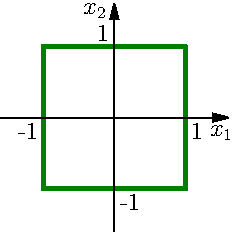
\includegraphics[width=3cm]{Cperron_1.pdf}
    \hspace{2cm}
    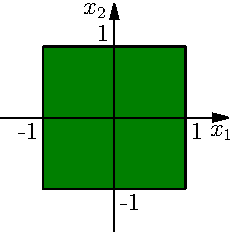
\includegraphics[width=3cm]{Cperron_2.pdf}
    \caption{$\mathcal{N} \cap \R^2$ et $\mathcal{B} \cap \R^2$}
\end{figure} 

  \item Par définition $f(u)=u$ ce qui signifie que $1$ est valeur propre de vecteur propre $u$. L'ensemble $\mathcal{S}$ des valeurs propres de $f$ (appelé son \emph{spectre}) est non vide, il contient au moins $1$.
  
  \item On veut montrer que le module d'une valeur propre est inférieure ou égale à $1$.
  \begin{enumerate}
     \item Soit $w$ un vecteur propre de valeur propre $\lambda$ et $\mu \in \C$ non nul.\newline Notons $v = \mu w \neq 0_F$. C'est encore un vecteur propre car 
\[
  f(v) = f(\mu w) = \mu f(w) = \mu (\lambda w) = \lambda (\mu w) = \lambda v.
\]

     \item \label{stabB} Soit $w = (z_1,\cdots,z_p)\in \mathcal{B}$. Par linéarité de $f$, la $j$-ème coordonnée de $f(w)$ est $a_{1 j}v_1 + \cdots + a_{p j} v_p$ avec 
\[
 |\underset{ >0}{\underbrace{a_{1 j}}}\,z_1 + \cdots + \underset{ >0}{\underbrace{a_{p j}}}\, z_p | \leq 
 a_{1 j}\,\underset{ \leq 1}{\underbrace{|z_1|}} + \cdots +  a_{p j}\,\underset{ \leq 1}{\underbrace{|z_p|}} \leq  a_{1 j} + \cdots + a_{p j} =  1 
\]
d'après I1b. Ceci étant valable pour tous les $j$, on en tire $f(v)\in\mathcal{B}$.

     \item Soit $w=(z_1,\cdots,z_p)$, notons $W = \max(|z_1|,\cdots,|z_p|)$. Alors $w\neq 0_F \Rightarrow W >0$. Il suffit de choisir $\mu = \frac{1}{W}$ pour que $\mu\,w \in \mathcal{N}$.
     
     \item Soit $\lambda$ une valeur propre. D'après c. et a., il existe $w =(z_1, \cdots, z_p) \in \mathcal{N}$ qui est un vecteur propre de valeur propre $\lambda$. Comme $\mathcal{N} \subset \mathcal{B}$, la question b. montre que 
\[
  \lambda w = f(w) \in \mathcal{B} \Rightarrow \forall j \in \llbracket 1,p \rrbracket,\; |\lambda z_j| \leq 1.
\]
Il existe un $j$ tel que $|z_j| = 1$ car $w \in \mathcal{N}$. On en déduit $|\lambda| \leq 1$.
  \end{enumerate}

  \item Soit $\lambda$ une valeur propre de module $1$.
    \begin{enumerate}
      \item Comme dans la question précédente, il existe $w =(z_1, \cdots, z_p) \in \mathcal{N}$ (d'après 3.c. et 3.a.) qui est un vecteur propre de valeur propre $\lambda$. 
      
      \item Il existe $j$ tel que $|z_j| = 1$ et $|z_i|\leq 1$ pour tous les $i$ car $w=(w_1,\cdots,w_p) \in \mathcal{N}$. Considérons la $j$-ème coordonnée de $f(w)$:
\[
 a_{1 j}z_1 + \cdots + a_{p j} z_p = \lambda z_j.
\]
Divisons par $\lambda z_j$ qui est non nul car de module $1$. On en tire
\[
 a_{1 j}u_1 + \cdots + a_{p j} u_p = 1
 \text{ avec }
 u_k = \frac{z_k}{\lambda z_i} \Rightarrow |u_k| = \frac{|z_k|}{|\lambda z_i|} \leq 1.
\]
On conclut alors que $u_k = 1$ pour tous les $k$ avec la question I.3.b. car 
\[
  a_{1 j} + \cdots + a_{p j} = 1.
\]
En considérant $k =j$, on obtient $\lambda = 1$. Ceci prouve que $1$ est \emph{la seule valeur propre de module 1}. Pour tous les autres $k$, on obtient $z_k = z_j$.\newline
On peut noter que cela entraine $w = z_j u$ ce qui est utile dans la question suivante.
      
      \item  Remarquons que $v\in  \ker (f-\Id_F) \Leftrightarrow f(v)=v$. Comme $f(u)=u$ par hypothèse, $u\in  \ker (f-\Id_F)$ donc $\Vect(u)\subset  \ker (f-\Id_F)$.\newline
Soit $v$ non nul dans $\ker (f-\Id_F)$. D'après 3.c. et 3.a., il existe $\mu >0$ tel que $\mu v = (z_1, \cdots, z_p)$ soit un vecteur propre dans $\mathcal{N}$ de valeur propre $1$. D'après la question précédente, il existe $j$ tel que $\mu v = z_i u \in \Vect(u)$. On en tire l'autre inclusion donc
\[
 \ker(f-\Id_F) = \Vect(u).
\]
 \end{enumerate}
\end{enumerate}


\subsection*{Partie III. Hyperplan supplémentaire stable.}
\begin{enumerate}
 \item 
\begin{enumerate}
 \item Si $g(x)=0$ alors $g^(x)=0$ donc $\ker g \subset \ker g^2$ donc $\dim(\ker g) \leq \dim(\ker g^2)$.\newline
Pour la deuxième inégalité, considérons $g'$ la restriction de $g$ à $\ker g^2$. Elle prend ses valeurs dans $\ker g$ donc $\rg g' \leq \dim(\ker g)$ et son noyau est $\ker g$. Appliquons à $g'$ le théorème du rang :
\[
 \dim(\ker g^2) = \dim(\ker g) + \rg(g')\leq 2\dim(\ker g).
\]

 \item \label{equiv} On sait que $\ker g \subset \ker g^2$ et $\Im g^2 \subset \Im g$ pour tout endomorphisme $g$.\medskip
\begin{itemize}
  \item Supposons $\Im g \oplus \ker g = E$ et montrons que $\Im g \subset \Im g^2$.\newline
Soit $x=g(y)\in \Im g$, décomposons $y$ en $y=a+b$ avec $a\in \ker g$ et $b=g(c)\in \Im g$. On en tire $x=g^2(c)\in \Im g^2$ donc $\Im g = \Im g^2$.\smallskip

  \item Supposons $\Im g = \Im g^2$ et montrons que $\ker g = \ker g^2$.\newline
  L'égalité des deux images entraine l'égalité des dimensions des deux images. Le théorème du rang entraine l'égalité des dimensions des deux noyaux. Comme $\ker g \subset \ker g^2$, l'égalité des dimensions entraine l'égalité des espaces.\smallskip
  
  \item Supposons $\ker g^2 = \ker g$ et montrons que $\Im g \oplus \ker g = E$. \newline
Si $x \in \Im g \cap \ker g$, il existe $y$ tel que $x=g(y)$ et $g(x)=0$. Alors $g^2(y)=0$ donc $y\in \ker g^2 \subset \ker g$ donc $g(y)=x=0$. L'intersection est réduite au vecteur nul donc $\dim (\Im g + \ker g) = \dim \Im g + \dim \ker g = \dim E$ à cause du théorème du rang. D'où $\Im g + \ker g = E$ puis $\Im g \oplus \ker g = E$.
\end{itemize}\smallskip
Les trois implications prouvées au dessus montrent circulairement l'équivalence
\[
  \Im g \oplus \ker g = E \Leftrightarrow \Im g^2 = \Im g \Leftrightarrow \ker g^2 = \ker g .
\]
\end{enumerate}

 \item Notons $g = f - \Id_F$ de sorte que $f=\Id_F +g$. La formule du binôme est valable pour une somme de deux endomorphismes qui commutent:
\begin{displaymath}
 f^n = \Id_F + \binom{n}{1}g + \binom{n}{2}g^2 + \binom{n}{3}g^3 + \cdots 
\end{displaymath}
On sait d'après II.4.c que $\ker g = \Vect(u)$ donc $\dim(\ker g) = 1$. Si $\dim(\ker g^2) =2$ l'inclusion entre les deux noyaux est stricte et il existe un $w \in \ker g^2$ avec $w \notin \ker g$. On a donc $f(w)\neq w$ et $g^2(w)=0$. Le vecteur $v$ n'est pas forcémént dans $\mathcal{B}$ mais, comme il est non nul, il existe $\mu >0$ tel que $v = \mu w =(z_1,\cdots,z_p)\in \mathcal{N} \subset \mathcal{B}$ et qui vérifie les mêmes propriétés. L'expression de $f^n(v)$ se réduit alors à
\begin{displaymath}
 f^n(v) = v + \binom{n}{1}g(v) + 0 = v +n(f(v)-v) .
\end{displaymath}
Ceci entre en contradiction avec le fait que $\mathcal{B}$ est stable par $f$ (partie II question III.b). En effet il existe un indice $j$ tel que la $j$-ème coordonnée de $v$ soit différente de la $j$-ème coordonnée de $f(v)$. Pour ce $j$, la suite des $j$-ème coordonnés de $f^n(v)$ va diverger vers $+\infty$ ou $-\infty$ et ne sera pas bornée par $1$. 
Ceci prouve que $\ker g^2 = \ker g$.

\item Toujours avec $g = f - \Id_F$, la question 1.a. montre que 
\[
  \ker(f - \Id_F)^2 = \ker(f- \Id_F) \Rightarrow \Im (f- \Id_F) \oplus \ker (f- \Id_F) = E. 
\]
Comme $\ker (f - \Id_F) =\Vect(u)$ est une droite vectorielle, $\Im (f - \Id_F)$ est un hyperplan supplémentaire noté $H$.\newline
Il est stable par $f$ car si $x\in H$, il existe $y \in F$ tel que
\begin{displaymath}
 x = f(y) -y \Rightarrow f(x) = f^2(x)-f(x)=(f-\Id_F)(f(x))=g(x)\in H .
\end{displaymath}
 
 \item 
\begin{enumerate}
 \item Il s'agit d'une question de cours. Soit $v$ un vecteur qui n'est pas dans l'hyperplan $\ker \phi = \ker \psi$ alors $\psi(v)$ et $\phi(v)$ sont non nuls et la droite $\Vect(v)$ est un supplémentaire de cet hyperplan. En décomposant dans $\ker \psi \oplus \Vect(v)$, on vérifie que $\phi = \frac{\phi(v)}{\psi(v)}\,\psi$.

 \item Comme $H$ est un hyperplan, il existe une forme linéaire $\gamma_1$ telle que $H=\ker \gamma_1$ avec $\gamma_1(u)\neq 0$ car $u$ n'est pas dans $H$. On peut poser $\gamma = \frac{1}{\gamma_1(u)}\gamma_1$ pour assurer que $\gamma(u)=1$.\newline
Notons $\gamma' = \gamma \circ f$. C'est encore une forme linéaire et elle n'est pas nulle car $\gamma'(u) = 1$. La stabilité de $H$ par $f$ entraine que $H \subset \ker \gamma'$. Comme il sont de même dimension, les deux hyperplans sont égaux. Il existe donc un réel $\lambda$ tel que $\gamma' = \lambda \gamma$. De plus $\lambda=1$ car $\gamma(u)=\gamma'(u)$. 
  
  \item Décomposons $v \in F$ dans $\Vect(u) \oplus H$. Il existe $\mu \in \C$ et $h \in H = \ker \gamma$ tel que 
\[
  v = \lambda u + h \Rightarrow \gamma(v) = \lambda \gamma(u) \Rightarrow p_{\Vect(u)\, H}(v) = \lambda u = \gamma(v)u \text{ car } \gamma(u) = 1.
\]

\end{enumerate}
\end{enumerate}

\subsection*{Partie IV. Convergence.}
\begin{enumerate}
 \item  Utilisons la formule du binôme pour l'endomorphisme 
\[
  f^n = \left(\lambda \Id_F + (f -\lambda \Id_F) \right)^n
\]
car $\lambda \Id_F$ commute avec $f -\lambda \Id_F$. Prenons la valeur en $v \in \ker(f- \lambda \Id_F)^p$:
\[
f^n(v) = \lambda ^n v + \sum_{k=1}^{p-1}\binom{n}{k}\lambda^{n-k}\,(f-\lambda\Id_F)^k(v)  
\]
car $(f-\lambda\Id_F)^k(v)=0$ pour $k\geq p$. D'après II., $|\lambda|<1$ car c'est une valeur propre autre que $1$. De I.1., on déduit que toutes les suites numériques en jeu (pour chaque $k$ et chaque coordonnée) dans la suite de vecteurs $(f^n(x))_{n \geq p}$ convergent vers $0$.
 
 \item Soit $\lambda$ une valeur propre telle que $\ker(f - \lambda \Id_F)^p \subset H$ et $v\neq 0_F$ un vecteur propre associé. 
\[
\left.
\begin{aligned}
  &v \in \ker(f - \lambda \Id_F) \subset \ker(f - \lambda \Id_F)^p \subset H \\
  &H \cap \ker(f - \Id_F) = \left\lbrace 0_F\right\rbrace
\end{aligned}
\right\rbrace \Rightarrow
 f(v) \neq v \Rightarrow \lambda \neq 1 \Rightarrow |\lambda| < 1  
\]
car d'après II. $|\lambda|\leq 1$ et $\lambda \neq 1 \Rightarrow |\lambda| < 1$.

 \item Comme $\Vect(u) \oplus H = F$, tout vecteur $v$ se décompose en
\begin{displaymath}
 v = \gamma(v) u + h \text{ avec } h = \in H = \ker \Gamma.
\end{displaymath}
De plus, d'après la propriété admise, $h$ se décompose en une somme $h = v_1 + \cdots + v_r$ avec $v_k \in \ker(f-\lambda_k)^p$. La question 2 montre que les suites de coordonnées des $f^n(v_k)$ convergent vers $0$. La seule composante qui contribue réellement à la limite est celle dans $\Vect(u)$ qui est constante. Toutes les suites de coordonnées des $f^n(v)$ convergent vers la même valeur $\gamma(v)$.
\end{enumerate}
